\documentclass[zihao=-4]{ctexart}
\usepackage[normalem]{ulem}
\useunder{\uline}{\ul}{}
%********************导言区宏包引入********************
\usepackage{xeCJK}
\usepackage{amssymb}
\usepackage{amsmath}
\usepackage{listings} %代码
\usepackage{graphicx}
\usepackage{multicol} %回车换段
\usepackage{xcolor}
\usepackage{geometry} %页面设置
\usepackage{fontspec}
\usepackage{setspace}
\usepackage{times}
\usepackage{fancyhdr} %页眉页脚
\pagestyle{fancy}
\usepackage{float} %表格位置
\usepackage{titlesec} %设置
\usepackage{titletoc}
\usepackage{ctex}
\usepackage{gbt7714}    %控制参考文献格式为国标
\usepackage{multirow}
\usepackage{booktabs}   %表格相关
\usepackage{setspace}   %设置行距
\usepackage{caption} %caption
\usepackage{subcaption} %子图的caption
\usepackage{changepage} %左右缩进
\usepackage{xurl}
\def\UrlBreaks{%
    \do\/%
    \do\a\do\b\do\c\do\d\do\e\do\f\do\g\do\h\do\i\do\j\do\k\do\l%
    \do\m\do\n\do\o\do\p\do\q\do\r\do\s\do\t\do\u\do\v\do\w\do\x\do\y\do\z%
    \do\A\do\B\do\C\do\D\do\E\do\F\do\G\do\H\do\I\do\J\do\K\do\L%
    \do\M\do\N\do\O\do\P\do\Q\do\R\do\S\do\T\do\U\do\V\do\W\do\X\do\Y\do\Z%
    \do0\do1\do2\do3\do4\do5\do6\do7\do8\do9\do=\do/\do.\do:%
    \do\*\do\-\do\~\do\'\do\"\do\-}
\urlstyle{same}


% for 代码
\definecolor{mygreen}{rgb}{0,0.6,0}
\definecolor{mygray}{rgb}{0.5,0.5,0.5}
\definecolor{mymauve}{rgb}{0.58,0,0.82}
\definecolor{myblue}{rgb}{0, 0, 1}


\graphicspath{ {include_picture/} }
\let\algorithm\relax
\let\endalgorithm\relax
\usepackage[ruled,vlined]{algorithm2e}%[ruled,vlined]{
\usepackage{algpseudocode}
\renewcommand{\algorithmicrequire}{\textbf{Input:}} 
\renewcommand{\algorithmicensure}{\textbf{Output:}}
%\renewcommand\thepage{\zihao{-5} ~\arabic{page}~}%页码字号

%定义两个arg
\DeclareMathOperator*{\argmax}{arg\,max}
\DeclareMathOperator*{\argmin}{arg\,min}
\DeclareCaptionLabelSeparator{mysep}{\space\space}  %自定义caption格式
\captionsetup[figure]{font={small}, labelfont=bf, labelsep=mysep, textfont=bf}   %图片caption格式
\captionsetup[table]{font={small}, labelfont=bf, labelsep=mysep, textfont={bf}}   %表格caption格式
\bibliographystyle{gbt7714-numerical} %修改了title斜体内容

\usepackage[colorlinks,bookmarksopen,bookmarksnumbered,citecolor=blue, urlcolor=blue]{hyperref}
\hypersetup{
    linkcolor=black
}

%********************导言区宏包引入********************
% Use TeX Live fonts; original proprietary font files are not redistributed.
\setmainfont{TeX Gyre Termes}
\setmonofont{TeX Gyre Cursor}
\setCJKfamilyfont{hwzs}{FandolSong-Regular}
\newcommand{\zhongsong}{\CJKfamily{hwzs}}
\setCJKfamilyfont{hwxw}{FandolKai-Regular}
\newcommand{\xinwei}{\CJKfamily{hwxw}}

%********************中文字号设置********************
%\newcommand{\chuhao}{\fontsize{42pt}{\baselineskip}\selectfont}
\newcommand{\chuhao}{\fontsize{42pt}{0}}
\newcommand{\xiaochu}{\fontsize{36pt}{0}}
\newcommand{\yihao}{\fontsize{28pt}{0}}
\newcommand{\erhao}{\fontsize{21pt}{0}}
\newcommand{\xiaoer}{\fontsize{18pt}{0}}
\newcommand{\sanhao}{\fontsize{16pt}{0}}
\newcommand{\sihao}{\fontsize{14pt}{0}}
\newcommand{\xiaosi}{\fontsize{12pt}{0}}
\newcommand{\wuhao}{\fontsize{10.5pt}{0}}
\newcommand{\xiaowu}{\fontsize{9pt}{0}}
\newcommand{\liuhao}{\fontsize{8pt}{0}}
\newcommand{\qihao}{\fontsize{5.25pt}{0}}

% 个人信息 自定义命令 固定长度下划线
\newcommand\ful[2][4cm]{\underline{\makebox[#1][c]{#2}}}
%********************中文字号设置********************


%********************代码段********************
% https://www.cnblogs.com/PiaYie/p/15720770.html
\lstset{ %
  backgroundcolor=\color{white},   % choose the background color; you must add \usepackage{color} or \usepackage{xcolor}
  basicstyle=\footnotesize,        % the size of the fonts that are used for the code
  breakatwhitespace=false,         % sets if automatic breaks should only happen at whitespace
  breaklines=true,                 % sets automatic line breaking
  captionpos=bl,                    % sets the caption-position to bottom
  commentstyle=\color{mygreen},    % comment style
  deletekeywords={...},            % if you want to delete keywords from the given language
  escapeinside={\%*}{*)},          % if you want to add LaTeX within your code
  extendedchars=true,              % lets you use non-ASCII characters; for 8-bits encodings only, does not work with UTF-8
  frame=single,                    % adds a frame around the code
  keepspaces=true,                 % keeps spaces in text, useful for keeping indentation of code (possibly needs columns=flexible)
  keywordstyle=\color{blue},       % keyword style
  %language=Python,                 % the language of the code
  morekeywords={*,...},            % if you want to add more keywords to the set
  numbers=left,                    % where to put the line-numbers; possible values are (none, left, right)
  numbersep=5pt,                   % how far the line-numbers are from the code
  numberstyle=\tiny\color{mygray}, % the style that is used for the line-numbers
  rulecolor=\color{black},         % if not set, the frame-color may be changed on line-breaks within not-black text (e.g. comments (green here))
  showspaces=false,                % show spaces everywhere adding particular underscores; it overrides 'showstringspaces'
  showstringspaces=false,          % underline spaces within strings only
  showtabs=false,                  % show tabs within strings adding particular underscores
  stepnumber=1,                    % the step between two line-numbers. If it's 1, each line will be numbered
  stringstyle=\color{orange},     % string literal style
  tabsize=2,                       % sets default tabsize to 2 spaces
  literate={-}{{\textendash}}{1}
  %title="No name code"                   % show the filename of files included with \lstinputlisting; also try caption instead of title
}
%********************代码段********************


%********************页边距设置********************
\geometry{left=3cm,right=2cm,top=2.5cm,bottom=2.5cm}
\geometry{a4paper} % xsp 2023/3/7: 调整纸张大小为A4
%********************页边距设置********************

%********************段间距设置********************
\newcommand{\setParDis}{\setlength {\parskip} {0pt} }
%请在每部分使用这个
%********************段间距设置********************

%********************

\begin{document}
%********************页眉页脚设置********************
\lhead{}%设置左页眉为空
\rhead{}%设置左页眉为空
\setlength{\headwidth}{\textwidth}% 2023/3/3 XSP: 页眉长度适应文本
%********************页眉页脚设置********************


%********************标题格式设置********************

%\setcounter{secnumdepth}{0}%该命令取消了章标题前数字label

\CTEXsetup[name={,、},number={\chinese{section}}]{section}
\CTEXsetup[name={（,）},number={\chinese{subsection}}]{subsection}
\CTEXsetup[name={,.},number={\arabic{subsubsection}}]{subsubsection}% 不加会导致目录格式错误
% 设置subsubsection等格式
% \titleformat{\section}[block]{\sanhao\bfseries\centering}{\chinese{section}、}{0pt}{}[]
% \titleformat{\subsection}[block]{\sihao\bfseries}{（\chinese{subsection}）}{0pt}{}[]
% \titleformat{\subsubsection}[block]{\xiaosi\bfseries}{\arabic{subsubsection}、}{0pt}{}[]
\titleformat{\section}[block]{\sanhao\heiti\centering}{\chinese{section}、}{0pt}{}[]    % XSP 2023/3/3:
\titleformat{\subsection}[block]{\sihao\heiti}{（\chinese{subsection}）}{0pt}{}[]       %   将正文标题字体由加粗
\titleformat{\subsubsection}[block]{\xiaosi\heiti}{\arabic{subsubsection}.}{0pt}{}[]   % 修改为黑体。
\titlespacing{\section}{0pt}{25pt}{12pt}
\titlespacing{\subsection}{0pt}{7pt}{7pt}
\titlespacing{\subsubsection}{0pt}{5pt}{4pt}

\titlecontents{section}[1.6em]{\addvspace{2pt}\filright}
{\contentspush{\thecontentslabel\hspace{0.8em}}}
{}{\titlerule*[8pt]{.}\contentspage}

\titlecontents{subsection}[3.2em]{\addvspace{2pt}\filright}
{\contentspush{\thecontentslabel\hspace{0.8em}}}
{}{\titlerule*[8pt]{.}\contentspage}

\titlecontents{subsubsection}[6.4em]{\addvspace{2pt}\filright}
{\contentspush{\thecontentslabel\hspace{0.8em}}}
{}{\titlerule*[8pt]{.}\contentspage}
%********************标题格式设置********************

%\setcounter{section}{-3}  %标题计数器
%\stepcounter{section}

%*******************行间距段前段后*******************
\linespread{1.8}
%行间距为实际行间距乘以1.2,如此处实际为1.5倍行距
\setlength{\parskip}{0.5\baselineskip}
%*******************行间距段前段后*******************



% Identifying course cover removed during archival cleanup.
\renewcommand{\headrulewidth}{0pt}
\pagenumbering{roman} %摘要目录页小写罗马

\xiaosi
% \section*{摘要}
% \begin{spacing}{1.5}
%   \setParDis %设置段间距为 0
% 摘要正文

% \end{spacing}
    
% \textbf{关键词：}关键词1，关键词2，关键词3，关键词4，关键词5

% \newpage
% \section*{\textbf{Abstract}} % XSP 2023/3/8: Abstract 加粗
% \begin{spacing}{1.5}
% \begin{adjustwidth}{0.42cm}{0.42cm}
%   \setParDis %设置段间距为 0

% \qquad Abstract content.

% \textbf{Keywords: Keywords 1, Keywords 2, Keywords 3, Keywords 5, Keywords 6}
% \end{adjustwidth}
% \end{spacing}



%********************摘要部分********************


%********************目录部分********************
\clearpage
\tableofcontents
\clearpage
%********************目录部分********************


\renewcommand{\headrulewidth}{0.4pt} %恢复页眉装饰线

%********************正文页眉部分********************
%\lhead{} 
\chead{\xiaowu \CourseName 大作业报告} %设置居中页眉
%********************正文页眉部分********************

\pagenumbering{arabic} %正文页码从1开始，用阿拉伯数字
\setcounter{page}{1} 

\section{CUDA模型}
\setParDis %设置段间距为 0
\begin{spacing}{1.5}

CUDA（Compute Unified Device Architecture）是由NVIDIA开发的并行计算平台和编程模型，使开发人员能够充分利用GPU的强大并行计算能力。

\subsection{CUDA硬件模型}

CUDA硬件模型主要由以下几个关键组件组成：GPU处理集群（GPU Processing Clusters，GPC）、纹理处理集群（Texture Processing Clusters，TPC）、流式多处理器（Streaming Multiprocessors，SM）和CUDA核心（Streaming Processor，SP）。

GPC是CUDA GPU架构中最高级别的结构单元。每个GPC包含若干TPC和其他一些共享资源，例如L2缓存。GPC负责处理大量并行任务，实现高吞吐量的计算能力。一个GPU通常包含多个GPC，从而可以并行处理更多的任务。每个GPC内部分布着多个TPC，TPC是次一级的集群，主要负责处理纹理相关的计算任务。TPC还包含若干SM，它是CUDA硬件架构中的基本计算单元。图\ref{GA100_structure}是来自NVIDIA Ampere架构白皮书$^{[1]}$中的GPU核心结构图，由于我使用的GPU是Ampere架构的，因此我选用了同样的架构。

\begin{figure}[H] %H为当前位置，!htb为忽略美学标准，htbp为浮动图形
    \centering %图片居中
    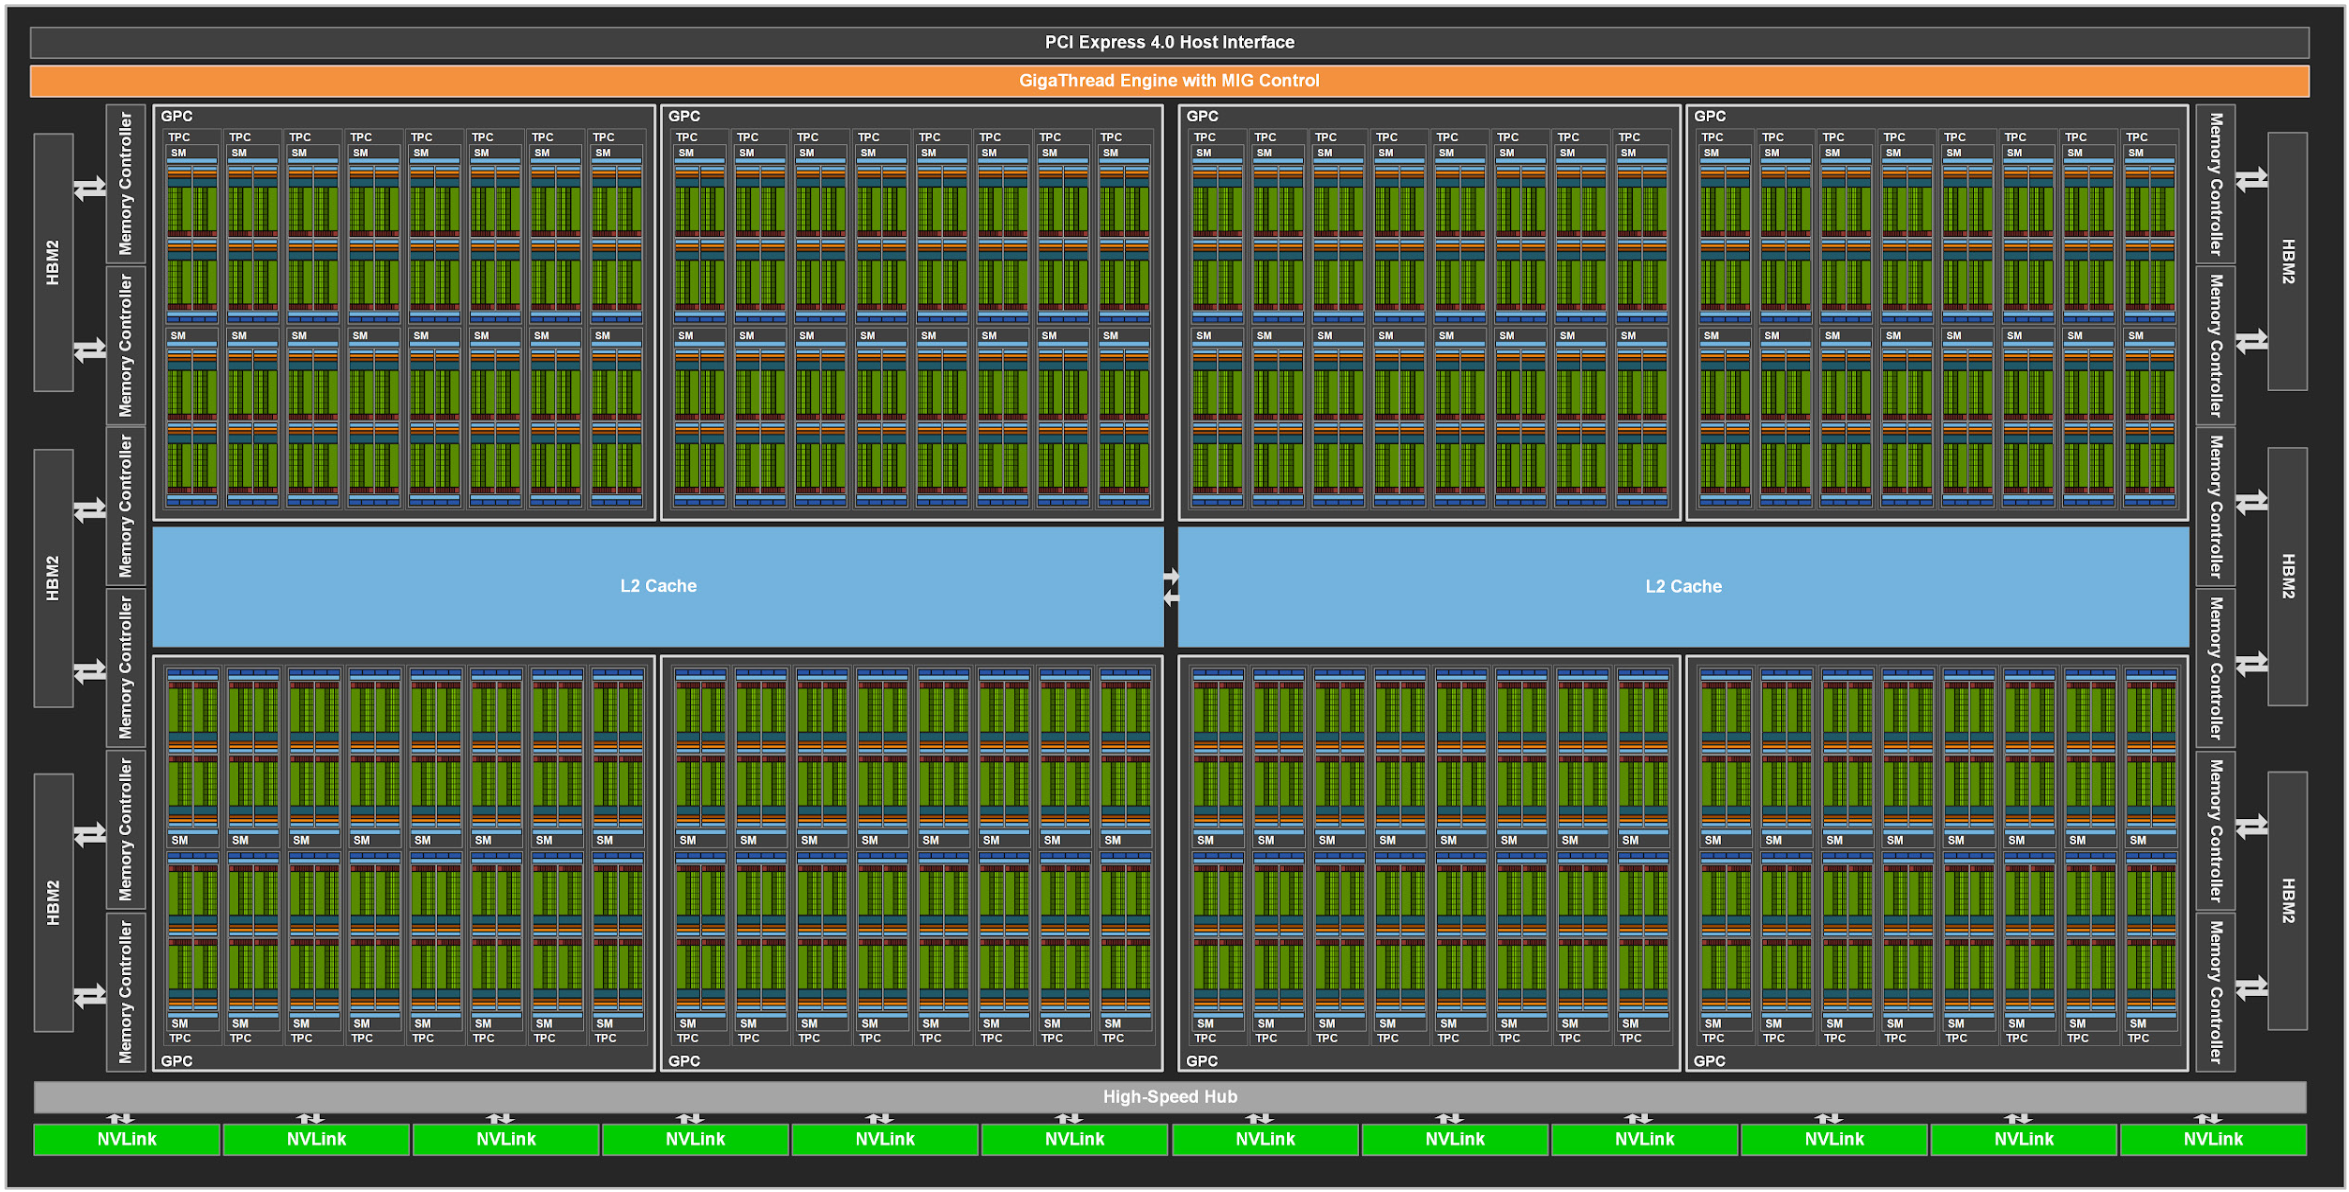
\includegraphics[width=0.8\textwidth]{include_picture/GA100_arch.png} %插入图片，[]中设置图片大小，{}中是图片文件名
    \caption{GA100核心全景结构图} %最终文档中希望显示的图片标题
    \label{GA100_structure} %用于文内引用的标签
\end{figure}

如图\ref{GA100_SM_structure}所示，每个流式多处理器包含若干CUDA核心、调度器（scheduler）、寄存器文件、共享内存和其他辅助硬件。SM负责执行具体的CUDA线程块（thread blocks）。CUDA核心是最基本的计算单元，执行CUDA程序中的线程指令。每个SM中的CUDA核心可以执行浮点运算（FP32、FP64）和整数运算（INT32），以及深度学习加速运算（Tensor Cores）。每个SM包含的CUDA核心数量通常较多，这使得GPU能够高效地执行并行计算任务。需要注意的是，当我们提到一个GPU的CUDA核心总数时，这通常指的是FP32核心的总数，因为FP32运算是GPU中最常见的运算类型。

\begin{figure}[H] %H为当前位置，!htb为忽略美学标准，htbp为浮动图形
    \centering %图片居中
    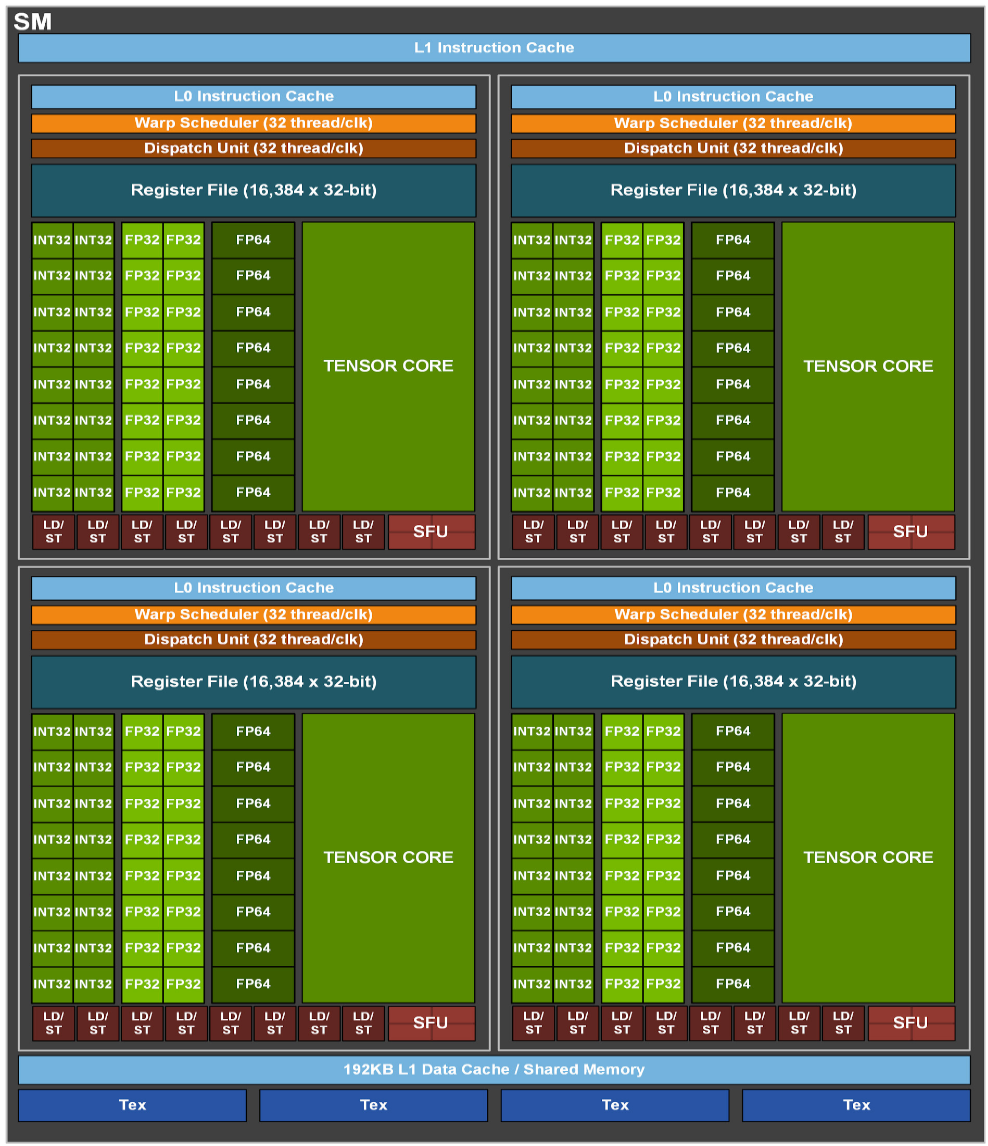
\includegraphics[width=0.8\textwidth]{include_picture/GA100_SMarch.png} %插入图片，[]中设置图片大小，{}中是图片文件名
    \caption{GA100核心SM结构图} %最终文档中希望显示的图片标题
    \label{GA100_SM_structure} %用于文内引用的标签
\end{figure}

在硬件层级关系中，GPC包含多个TPC，TPC包含多个SM，而SM包含多个CUDA核心。这个层级结构确保了CUDA GPU能够高效地处理大规模并行计算任务。例如，假设一个CUDA GPU具有4个GPC，每个GPC包含2个TPC，每个TPC包含4个SM，而每个SM包含128个CUDA核心。这意味着该GPU总共有4096个CUDA核心。这种架构使得GPU能够高效地执行并行计算任务，并在各种应用场景中提供卓越的性能。

\subsection{CUDA存储模型图}

CUDA的存储架构是理解CUDA编程的关键，它决定了数据如何在主机（Host）和设备（Device）之间传输，以及如何在设备内存之间访问和共享。CUDA存储架构包括多种类型的内存，每种内存都有其特定的用途和访问机制。这些内存类型包括全局内存、常量内存、纹理内存、共享内存、寄存器和局部内存。理解这些存储类型与CUDA硬件结构的对应关系，可以帮助更好地优化CUDA程序。

\begin{figure}[H] %H为当前位置，!htb为忽略美学标准，htbp为浮动图形
    \centering %图片居中
    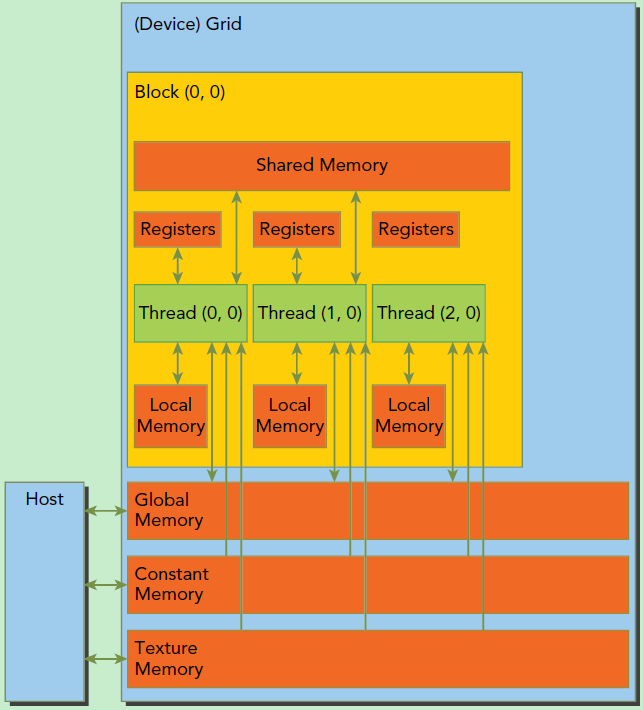
\includegraphics[width=0.8\textwidth]{include_picture/CUDA_mem.png} %插入图片，[]中设置图片大小，{}中是图片文件名
    \caption{CUDA存储模型} %最终文档中希望显示的图片标题
    \label{cuda_mem} %用于文内引用的标签
\end{figure}

全局内存是设备内存中容量最大的一部分，可以由所有线程访问。全局内存用于存储需要在多个线程块之间共享的数据。尽管其访问速度较慢，但由于其容量大，适合存储大量数据。在硬件结构中，全局内存位于GPU的所有流式多处理器（SM）之外，是一个共享的资源。全局内存的数据传输需要通过cudaMemcpy函数在主机和设备之间进行。图\ref{cuda_mem}中，最底层的全局内存是连接主机和设备的重要桥梁。

常量内存是只读内存，专门用于存储在整个核函数执行过程中不会改变的值。其容量较小，但在所有线程访问相同位置时具有较低的访问延迟。常量内存的内容在核函数执行之前通过cudaMemcpyToSymbol从主机复制到设备。在硬件架构中，常量内存和全局内存一样，位于所有SM之外，由一个专门的单元进行管理。图\ref{cuda_mem}中展示了常量内存位于全局内存旁边，但其访问速度和模式有所不同。

纹理内存也是一种只读内存，主要用于图像处理和其他需要高效随机访问的数据场景。纹理内存通过专门的纹理单元访问，可以显著提高2D和3D图像数据的处理效率。在硬件结构中，纹理内存由TPC中的纹理单元管理。图\ref{cuda_mem}中，纹理内存紧邻全局内存和常量内存，表示其在设备内存架构中的位置。

共享内存是每个线程块内的所有线程共享的高速内存。共享内存具有低访问延迟，适用于需要频繁访问和修改的数据。每个线程块在执行核函数时会分配一定大小的共享内存，线程块内的所有线程可以高效地访问和通信。在硬件结构中，共享内存位于每个SM内部，由SM管理。图\ref{cuda_mem}中，共享内存位于线程块内部。

寄存器是每个线程专用的高速存储器，用于存储线程执行过程中需要频繁访问的变量。寄存器具有最快的访问速度，但数量有限。每个线程在执行时会分配一定数量的寄存器，用于存储局部变量。在硬件结构中，寄存器也是SM内部的一部分，每个SM管理其内部的所有寄存器。图\ref{cuda_mem}中，寄存器紧邻线程，显示了其与每个线程的紧密关系。

局部内存是每个线程的私有内存，用于存储线程的私有数据，如自动变量和超出寄存器数量限制的变量。尽管名为局部内存，它实际上是设备全局内存的一部分，因此访问速度较慢。在硬件结构中，局部内存与全局内存相同，由设备内存管理单元管理。图\ref{cuda_mem}中，局部内存位于每个线程下方，表示其在线程执行中的位置。

图\ref{cuda_mem}示展示了CUDA存储架构的各个层次，显示了不同类型的内存以及它们之间的关系。主机通过全局内存、常量内存和纹理内存与设备进行数据交互，而在设备内部，线程通过寄存器、局部内存和共享内存高效地处理数据。这种多层次的存储架构使得CUDA能够高效地执行大规模并行计算任务，充分利用GPU的计算能力。

\subsection{NVIDIA GPU架构演进}

NVIDIA GPU架构经历了多次演进，每一代架构都在性能、效率和功能上有显著提升。这些架构演进不仅增强了GPU的计算能力，还引入了许多新技术和新特性，使其在高性能计算和人工智能领域发挥了重要作用。

Fermi架构标志着NVIDIA GPU向通用计算平台的转变。Fermi引入了流式多处理器的概念，每个SM包含32个CUDA核心。这一架构支持ECC内存和C++编程，大幅提升了计算精度和编程便利性。此外，Fermi还引入了L1和L2缓存体系结构，提高了内存访问效率。

Kepler架构在Fermi的基础上进一步优化，主要特点是提高了能效比。每个Kepler SMX（增强型SM）包含192个CUDA核心。Kepler引入了动态并行和Hyper-Q技术，前者允许GPU内核函数调用其他内核函数，后者通过多重队列机制提高了多线程执行效率。这些改进使得Kepler架构在高性能计算和图形处理方面表现出色。

Maxwell架构注重优化电源效率和性能，每个SM包含128个CUDA核心。Maxwell引入了新的内存压缩技术，显著降低了内存带宽需求。这一架构的设计目标是提高每瓦特的性能，使得GPU在高性能和低功耗之间取得了良好的平衡。

Pascal架构带来了深度学习加速的新突破。Pascal引入了支持混合精度计算的Tensor Cores，显著提升了深度学习训练和推理的性能。Pascal还支持NVLink高速互联技术，提供了更高的带宽以实现多GPU之间的快速数据传输。这些特性使Pascal在AI和高性能计算领域取得了巨大的成功。

Volta架构进一步增强了Tensor Cores的性能，每个SM包含64个CUDA核心和8个Tensor Cores。Volta引入了新的可编程内存访问模式，极大地提高了计算效率。Volta架构在AI计算方面表现尤为突出，广泛应用于深度学习和科学计算领域。

Turing架构引入了RT Cores用于实时光线追踪和Tensor Cores用于AI加速，每个SM包含64个CUDA核心、8个Tensor Cores和2个RT Cores。Turing架构大幅提升了图形渲染和AI计算的性能，开启了实时光线追踪技术的新时代，使得游戏和图形应用能够呈现更加逼真的画面效果。

Ampere架构进一步增强了Tensor Cores和RT Cores的性能。每个SM包含128个CUDA核心、4个Tensor Cores和1个RT Core。Ampere架构支持第三代Tensor Cores，可以进行更高效的AI计算，新的RT Cores提供更快的光线追踪性能。此外，Ampere架构还引入了多实例GPU（MIG）技术，允许将一个GPU分割成多个独立的实例，以便更高效地利用GPU资源。Ampere架构在深度学习、科学计算和图形处理等多个领域表现出色。

Hopper架构（以GH100为例）相较于前代Amper架构（GA100），在多个方面进行了提升。首先，Hopper架构中的流式多处理器数量从128增加到144，每个SM中的FP32 CUDA核心数量也翻倍，从64个增加到128个。此外，Hopper引入了第四代Tensor Cores，支持更高效的深度学习计算。同时，Hopper架构支持最新的HBM3和HBM2e显存，带宽从1555GB/s提升至3352GB/s，极大提高了内存访问速度。L2缓存的容量也从40MB增加到50MB，进一步提升了数据存储和访问效率。

在硬件创新方面，Hopper架构引入了Tensor Memory Accelerator（TMA）。TMA是一种专用硬件单元，用于优化全局内存和共享内存之间的数据传输。与之前需要使用特殊指令进行异步内存复制不同，TMA能够在不增加线程负担的情况下高效执行异步拷贝操作。单个线程可以启动TMA操作，创建一个复制描述符，之后的地址生成和数据移动由TMA硬件处理。TMA不仅支持线性拷贝，还支持最多五维的张量操作，处理地址、步幅、边界检查等复杂任务，进一步提升了数据搬运的效率和灵活性。

Hopper架构还引入了一个新的层次结构——Thread Block Cluster。Thread Block Cluster可以看作是“Block of Blocks”，为编程提供了新的视角和更大的灵活性。Thread Block Cluster中的所有Block被调度到同一个GPC上，享有更快的本地同步和内存共享。在这种架构下，同一个Cluster中的Block可以直接读写其他Block的共享内存，形成了Cluster Distributed Shared Memory（DSMEM），这极大地优化了跨Block的数据交换和通信效率。

异步屏障（Asynchronous Barriers）是Hopper架构中的另一项重要特性。与传统的同步机制不同，异步屏障将同步过程分为两个步骤：首先，线程完成各自的任务后标记为“到达”（Arrive），这一操作是非阻塞的，可以自由执行其他任务；然后，所有线程执行完独立任务后触发“等待”（Wait），这一操作是阻塞的，直到所有线程都到达后才继续执行。这种机制提高了线程并发性，减少了等待时间。Hopper架构还引入了Asynchronous Transaction Barrier，用于实现单向内存复制和消息传递，进一步提升了数据移动效率。

\subsection{CUDA编程模型}

\subsubsection{CUDA核函数}

CUDA编程模型使开发人员能够利用GPU的并行计算能力，通过定义和调用核函数（kernel function）来执行大规模并行计算任务。核函数是CUDA程序的核心组件，定义了在GPU上执行的代码，并通过配置网格和线程块的维度来管理并行计算的规模和粒度。

核函数使用\_\_global\_\_修饰符定义，它在设备上执行，由主机调用。核函数的主要作用是在GPU上并行处理数据，每个线程执行相同的代码，但操作不同的数据元素。以下是一个简单的矩阵加法核函数示例：

\begin{lstlisting}[language=C++,title={核函数示例}]
__global__ void matrixAdd(float* A, float* B, float* C, int N) {
    int i = blockIdx.x * blockDim.x + threadIdx.x;
    if (i < N) {
        C[i] = A[i] + B[i];
    }
}
\end{lstlisting}

在这个核函数中，我们使用了CUDA提供的几个内置变量来确定每个线程在网格和线程块中的位置。blockIdx表示线程块在网格中的索引，blockDim表示每个线程块中的线程数量，threadIdx表示线程在线程块中的索引。这些内置变量帮助计算每个线程处理的数据元素的位置。此外，CUDA还提供了gridDim变量，用于表示网格中线程块的数量。

这个示例程序中所使用的线程块和网格都是一维的，blockIdx.x是当前线程块在一维网格中的索引，blockDim.x是每个线程块中线程的数量，threadIdx.x是当前线程在线程块中的索引。通过这三个变量的组合，可以唯一确定每个线程在整个网格中的全局索引i。这个全局索引i对应于一维数据结构中的位置。在CUDA编程中，网格和线程块可以是一维、二维或者三维的。使用一维的网格和线程块是最简单和常见的情况，适用于线性数据结构（如数组、向量）或简单的计算任务。

\subsubsection{其它常用函数}

在CUDA编程中，除了核函数外，还有一些常用的辅助函数，用于内存管理、数据传输和同步操作。这些函数是高效利用GPU计算资源的重要工具。以下是一些最常用的CUDA函数及其简要介绍。

cudaMalloc函数用于在设备（GPU）上分配内存。它的原型为cudaError\_t cudaMalloc(void **devPtr, size\_t size)。devPtr是一个指向指针的指针，用于存储分配的设备内存地址，size是要分配的内存大小（以字节为单位）。例如，以下代码在设备上分配一个浮点型数组：

\begin{lstlisting}[language=C++,title={设备内存分配示例}]
float *d_A;
size_t size = N * sizeof(float);
cudaError_t err = cudaMalloc((void **)&d_A, size);
if (err != cudaSuccess) {
    // 处理错误
}
\end{lstlisting}

cudaFree函数用于释放之前使用cudaMalloc分配的设备内存。其原型为cudaError\_t cudaFree(void *devPtr)，devPtr是指向要释放的设备内存的指针。

cudaMemcpy函数用于在主机（Host）和设备（Device）之间传输数据。它的原型为cudaError\_t cudaMemcpy(void *dst, const void *src, size\_t count, cudaMemcpyKind kind);。dst和src分别是目标和源内存地址，count是传输的数据大小（以字节为单位），kind指定传输的方向（如cudaMemcpyHostToDevice或cudaMemcpyDeviceToHost）。例如，以下代码将数据从主机传输到设备：

\begin{lstlisting}[language=C++,title={数据传输示例}]
float *h_A = (float *)malloc(size);
cudaMemcpy(d_A, h_A, size, cudaMemcpyHostToDevice);
\end{lstlisting}

在并行计算中，同步操作至关重要。CUDA提供了多个同步函数，用于控制核函数的执行顺序和数据一致性。cudaDeviceSynchronize函数用于在主机代码中同步设备操作，确保之前启动的所有核函数在继续执行主机代码之前完成。其原型为cudaError\_t cudaDeviceSynchronize(void)。

\_\_syncthreads是一个内置的线程块级别的同步函数，用于在线程块内同步所有线程。每个线程在继续执行之前，都会等待所有线程都到达同步点。这个函数在核函数内部使用。

\subsubsection{编程约束}

在CUDA编程中，有一些特定的约束和限制，这些限制由CUDA架构的硬件特性决定，理解这些限制有助于编写高效且稳定的CUDA程序。

首先，线程块的大小有严格的限制。每个线程块中的线程数不能超过1024个，且线程块可以是一维、二维或三维的。一维线程块的最大尺寸为1024，二维线程块的每个维度最大尺寸为1024，而三维线程块的每个维度最大尺寸为64。这意味着一个二维线程块可以是32x32（总计1024个线程），而一个三维线程块可以是8x8x16（总计1024个线程）。

网格的大小也有具体限制。一维网格的最大尺寸为$2^{31}-1$，二维网格的每个维度最大尺寸为65535，三维网格的每个维度最大尺寸同样为65535。这些限制确保了在不同维度配置网格时的灵活性和可扩展性。

在硬件资源方面，每个CUDA设备有固定数量的寄存器、共享内存和常量内存。每个线程最多可使用255个32位寄存器，每个流式多处理器（SM）内的32位寄存器总数为64K。共享内存是线程块内所有线程共享的高速内存，每个SM可用的共享内存总量通常为64KB到96KB，但在最新的架构（如Hopper架构）中，这个值可以达到164KB甚至228KB。常量内存的总大小通常为64KB，用于存储在核函数执行过程中不变的数据。

每个CUDA设备还有一些其他的限制。例如，warp的大小是固定的，每个warp包含32个线程。每个SM上同时可驻留的最大线程块数和warp数有限。例如，一个SM上最多可以驻留32个线程块和64个warp，总线程数限制为2048。每个设备能够同时运行的并发核函数（resident grids）数量也有限，不同设备的具体值可以在在官网上的\href{https://docs.nvidia.com/cuda/cuda-c-programming-guide/#compute-capabilities}{CUDA C程序设计指导}中的表格21中查阅。

\subsubsection{CUDA程序基本流程}

CUDA程序的基本流程可以通过主机（CPU）和设备（GPU）之间的协同工作来实现，主要包括数据传输、核函数调用和结果返回等步骤。整个流程可以分为四个主要步骤，如图\ref{cuda_flow}所示。

\begin{figure}[H] %H为当前位置，!htb为忽略美学标准，htbp为浮动图形
    \centering %图片居中
    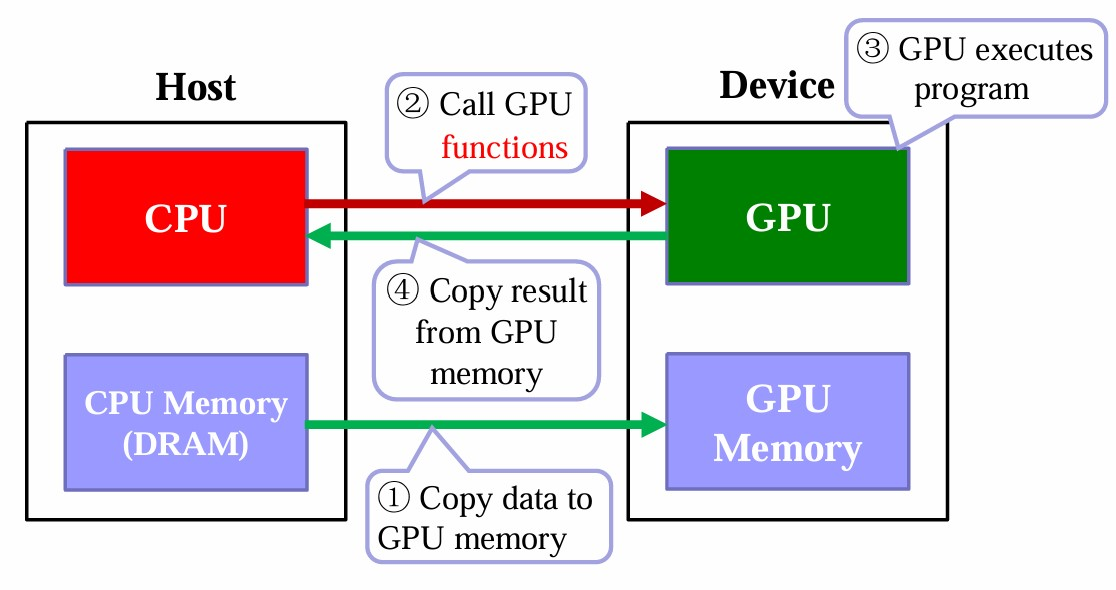
\includegraphics[width=0.8\textwidth]{include_picture/flow.jpg} %插入图片，[]中设置图片大小，{}中是图片文件名
    \caption{CUDA程序基本流程} %最终文档中希望显示的图片标题
    \label{cuda_flow} %用于文内引用的标签
\end{figure}

首先，程序在主机端开始，将需要处理的数据从主机内存复制到设备内存。这一步是通过调用cudaMemcpy函数来实现的，将数据从CPU内存传输到GPU内存。这一步确保了GPU能够访问和处理所需的数据，从而准备好进行并行计算。

接下来，主机端调用核函数，启动GPU的并行计算。核函数通过特殊的语法（如<<<blocks, threads>>>）配置网格和线程块的维度，以确定并行计算的规模。核函数在设备端执行，利用GPU的计算能力对数据进行处理。此时，GPU中的每个线程根据其索引处理不同的数据部分，实现高效的并行计算。

第三步，GPU执行核函数中的并行计算任务。GPU的各个线程协同工作，处理分配给它们的数据片段。核函数内部使用线程索引（如blockIdx、blockDim和threadIdx）来确定每个线程处理的数据位置，确保每个线程都有独立的工作负载。在核函数执行期间，主机端通常会等待GPU完成所有计算任务，可以通过同步函数（如cudaDeviceSynchronize）确保计算任务的正确完成。

最后一步，计算完成后，将结果从设备内存复制回主机内存。这一步再次使用cudaMemcpy函数，将处理结果从GPU内存传输回CPU内存。主机端接收到结果后，可以对其进行进一步的处理、验证或存储。这个数据传输过程确保了计算结果能够返回到主机，从而完成整个CUDA计算任务。

\subsubsection{主要优化方法}

在CUDA编程中，优化程序性能是充分利用GPU强大计算能力的关键。通过合理使用各种优化技术，可以显著提高CUDA程序的执行效率和性能。以下是一些常见的优化方法。

首先，合理使用共享内存是优化CUDA程序性能的重要手段之一。共享内存是每个线程块内的所有线程共享的高速内存，其访问延迟比全局内存低得多。因此，在需要频繁访问和修改的数据处理中，使用共享内存可以显著提高性能。例如，可以将需要频繁访问的数据从全局内存加载到共享内存中，线程间进行数据交换时直接使用共享内存，从而减少全局内存访问次数。

其次，使用常量内存优化只读数据访问。常量内存是专门用于存储在核函数执行过程中不会改变的数据，其访问延迟低且具有较高的带宽。如果核函数中的大部分线程都需要访问相同的只读数据，可以将这些数据存储在常量内存中，利用常量内存的缓存机制提高数据访问效率。

此外，确保全局内存访问的共线性也是一种有效的优化策略。在CUDA中，内存访问模式对性能有很大影响。全局内存访问的共线性是指连续的线程访问连续的内存地址，这种访问模式能够充分利用内存带宽，减少内存访问延迟。在编写核函数时，尽量保证线程按照共线性的方式访问内存，可以显著提高内存访问效率。

另一个优化方法是使用适当的线程块和网格配置。不同的CUDA设备具有不同的硬件资源限制，如每个SM（Streaming Multiprocessor）中的最大线程数、寄存器数量和共享内存大小。通过实验和性能分析，找到最优的线程块大小和网格配置，可以最大限度地利用GPU资源，提高计算效率。例如，对于需要大量计算的核函数，可以使用较大的线程块，以充分利用SM中的并行计算资源；对于内存访问密集的核函数，可以使用较小的线程块，以提高内存访问效率。

最后，减少分支和分支发散也是提高CUDA程序性能的重要方法。分支发散是指同一warp中的不同线程执行不同路径的情况，会导致性能下降。在编写核函数时，尽量减少条件语句和分支操作，或者将条件判断放在warp级别而不是线程级别，可以减少分支发散，提高执行效率。

\section{实验环境}

\subsection{实验环境简介}

本次实验在我的个人计算机上完成，CPU为AMD Ryzen 9 5900HX，8核16线程，基准速度3.30GHz，双通道内存共32GB，速度3200MHz，GPU为Ampere架构的NVIDIA GeForce RTX 3080 Laptop，16GB显存，具有48组流式多处理器，每组128个共6144个CUDA核心。在\href{https://www.nvidia.com/en-us/geforce/laptops/compare/30-series/}{官网}上能够查询到我GPU的CUDA Capability为8.6，图\ref{gpu_info}中展示了使用GPU-Z查看的更为详细的GPU硬件信息。

\begin{figure}[H] %H为当前位置，!htb为忽略美学标准，htbp为浮动图形
    \centering %图片居中
    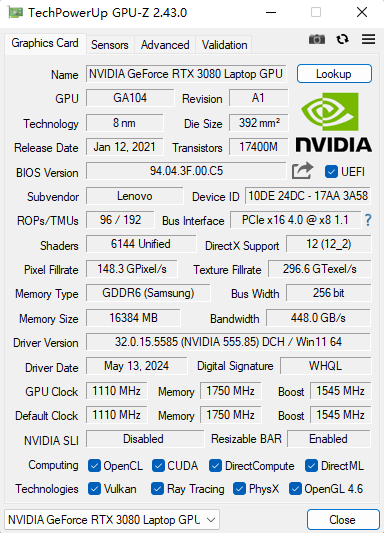
\includegraphics[width=0.6\textwidth]{include_picture/gpu_info.png} %插入图片，[]中设置图片大小，{}中是图片文件名
    \caption{GPU-Z查询到的GPU硬件信息} %最终文档中希望显示的图片标题
    \label{gpu_info} %用于文内引用的标签
\end{figure}

此外，一些软件环境的版本见下表。
\begin{table}[H]
\small
\caption{软件版本表}
\centering
\begin{tabular}{ll}
\hline  
\textbf{软件名} & \textbf{版本}\\ 
\hline  
Windows & 10.0.22000.2538\\
WSL & 2.1.5.0\\
WSL Linux内核 & 5.15.146.1-2\\
Ubuntu & 22.04.3 LTS\\
NVIDIA-SMI \& Driver & 555.42.03\\
Cuda compilation tools & V12.3.52\\
g++ & 11.4.0\\
\hline
\end{tabular} 
\end{table}

% TODO: 软件环境介绍

\subsection{环境配置流程}

为了完成本次作业，我需要为我所使用的个人计算机配置CUDA环境。斯坦福校方为本次作业准备了云服务器虚拟机，并提供了对应的配置脚本以及配置教程，以在其所提供的虚拟机中快速的配置CUDA环境。但我作为北航的学生，没有访问其所提供的虚拟机的权限，因而它的脚本和配置教程仅仅能作为参考，我需要结合我的具体运行环境进行配置。当然，或许还有使用docker的配置方式，但是我并没有使用这种方案，而是直接在我的WSL中进行配置。

环境配置和之后完成实验，均基于\href{https://github.com/stanford-cs149/asst3}{作业仓库}的提交fd0f705，这也是我完成作业时它最新的版本。在这个版本提供的配置脚本将会安装12.3版本的CUDA，和545.23.06版本的NVIDIA-SMI和Driver，这意味着我至少应该安装在此之上的版本。我查看我本地现有的版本，发现我NVIDIA-SMI和Driver的版本为512，其最高支持的CUDA版本为11.6。

由于我的系统版本与斯坦福提供的虚拟机一致，也就是说符合配置脚本中的需求，同为x86-64下的Ubuntu 22.04，因此我首先尝试直接运行配置脚本尝试环境的配置。第一次运行仓库中的环境配置脚本install.sh失败了，再次运行后安装脚本成功执行。执行完毕后，我通过nvcc查看到已经成功安装了12.3版本的CUDA，但是虽然安装了545版本的NVIDIA-SMI，但是Driver的版本仍为512，无法支持12.3版本的CUDA。

为此，我在WSL中卸载了我的GPU驱动程序，并回到宿主机，尝试使用宿主机中的GeForce Experience软件更新GPU驱动，但是以失败告终，在升级驱动时会报错。于是我去官网下载最新版本的驱动，并手动安装，成功。此时我进入WSL中，发现其中的NVIDIA-SMI和Driver已经同步得到了更新，版本均为555，能够运行12.3版本的nvcc编译产生的CUDA程序。

\section{翻译}

实验要求以及云服务器配置文档的翻译在“简单的CUDA渲染器”以及“AWS设置说明”两文件中，均提供了Markdown版本和PDF版本。

\section{实验一：SAXPY}

该部分是作业中的第一个实验，用于帮助学生熟悉CUDA编程模型。这部分的任务是使用CUDA重新实现实验一中的SAXPY函数。

\subsection{实验背景}

SAXPY函数是一种用于线性代数的基本操作，特别是在并行计算和数值计算中。它的主要目的是对向量进行缩放和相加。具体来说，它的操作是对两个向量X和Y进行元素级的操作，将向量X的每一个元素乘以常量a，然后加上向量Y中对应的元素，得到结果。

\subsection{实验代码浅析}

该部分的核心代码主要位于两个文件中，分别是主程序mian.cpp和saxpy.cu。

\subsubsection{主程序}

这个主程序的功能是测试和运行一个基于CUDA的SAXPY算法实现。程序首先设置默认的数组大小为100,000,000元素，并通过解析命令行参数允许用户指定数组大小。然后，程序初始化三个数组xarray、yarray和resultarray，并将xarray和yarray的每个元素设置为其索引值对 10 取余的结果，而resultarray的每个元素初始为0。

在初始化完成后，程序调用printCudaInfo函数来打印CUDA设备的信息，然后运行三次saxpyCuda函数来进行实际的SAXPY计算。每次计算中，saxpyCuda函数使用CUDA在GPU上执行SAXPY操作，将结果存储在resultarray中。最后，程序释放之前分配的数组内存并结束执行。

\subsubsection{算法实现}

saxpy.cu文件定义并实现了在GPU上运行的SAXPY算法。核心的CUDA内核函数saxpy\_kernel被标记为\_\_global\_\_，它在GPU上运行，并计算给定向量的SAXPY操作。每个线程根据其索引计算结果，并将其存储在结果数组中。

void saxpyCuda(int N, float alpha, float* xarray, float* yarray, float* resultarray)函数在CPU上运行，负责管理内存和调用CUDA内核，这也是在这个实验中需要实现的函数。首先，它计算需要处理的总字节数，并确定每个块中的线程数和所需的块数。然后，它在GPU上分配内存，并将输入数组从CPU复制到GPU。接着，它启动CUDA内核saxpy\_kernel，在GPU上并行执行计算。计算完成后，结果被复制回CPU，并记录和打印执行时间及带宽。最后，释放在GPU上分配的内存。

printCudaInfo函数打印当前机器上可用的CUDA设备信息，包括设备数量、名称、多处理器数量、全局内存大小和CUDA版本等详细信息。这个函数有助于了解执行环境中的GPU规格。

\subsection{实验过程}

该实验比较基础和简单，只需按照前文“CUDA程序基本流程”一节中所叙述的，完成设备内存的分配，将数据从主机拷贝到设备，调用核函数，最后再将结果从设备拷贝回主机即可。但是由于不太熟练，在这个简单的过程中一开始也犯了一些错误。

首先，在申请内存和进行数据拷贝时，一开始我忘了将使用的内存大小乘以sizeof (float)，导致了申请的内存长度不够，发生了内存的越界访问问题，使得程序在执行的过程中，会产生代码为700的错误，错误消息an illegal memory access was encountered。在看到这个错误之后，我进行排查，找到了问题所在，并进行了修改。

此外，在核函数执行完成后，我本应使用cudaDeviceSynchronize()进行同步，这导致我计算的执行时间惊人的快，几乎为0。正如实验说明中的叙述，由于主机和设备上的程序异步执行，如果我不进行同步，则此时只计算了API调用的时间，而没有计算核函数执行的时间。

\subsection{结果与结论}

在saxpy目录下完成本部分实验后，使用make进行编译，然后使用./cudaSaxpy进行执行，得到图\ref{saxpy_result}所示结果。

\begin{figure}[H] %H为当前位置，!htb为忽略美学标准，htbp为浮动图形
    \centering %图片居中
    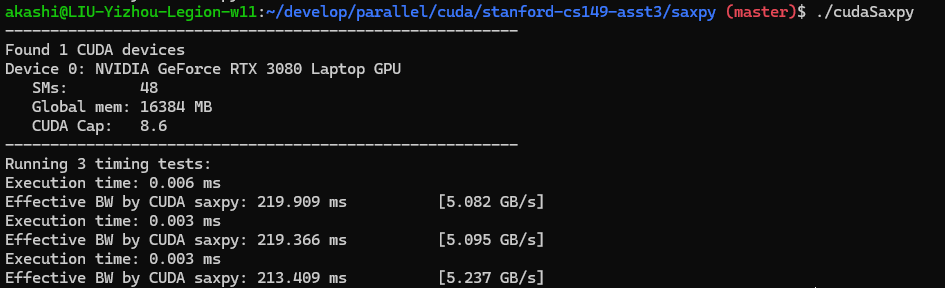
\includegraphics[width=0.8\textwidth]{include_picture/saxpy_result.png} %插入图片，[]中设置图片大小，{}中是图片文件名
    \caption{SAXPY实验程序执行结果} %最终文档中希望显示的图片标题
    \label{saxpy_result} %用于文内引用的标签
\end{figure}

通过图中展示的时间可以看出，GPU执行核函数的时间非常短，绝大多数时间都花费在了数据的传输上。

接下来回答实验说明中提出的问题。第一个问题是与基于顺序CPU的SAXPY实现的性能对比，由于我们没有完成这个部分，因此没有办法进行对比，但可以想象出，将会有很大的性能提升。

第二个问题第一部分是比较并解释由两组计时器提供的结果之间的差异。通过图中展示的时间可以看出，GPU执行核函数的时间非常短，绝大多数时间都花费在了数据的传输上。这说明GPU高度并行使得计算时间大幅缩短，但受限于内存、总线等设备的限制，在数据传输上需要消耗大量的时间。并且在实际的工作过程中，实际的数据传输速率受到各种因素影响，往往与理论上限仍有差距。

% 2*2四张子图示意
\begin{figure}[htbp]
  \begin{subfigure}{0.38\textwidth}
    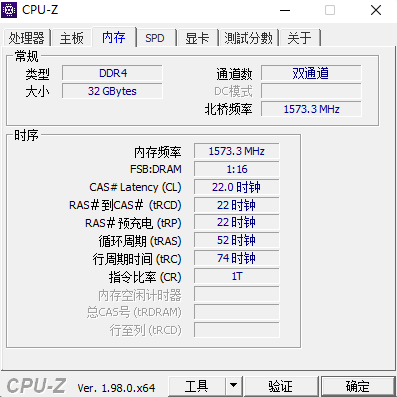
\includegraphics[width=\linewidth]{include_picture/mem_info.png}
    \caption{内存信息} \label{mem_info}
  \end{subfigure}%
  \hspace*{\fill}   % maximize separation between subfigures
  \begin{subfigure}{0.58\textwidth}
    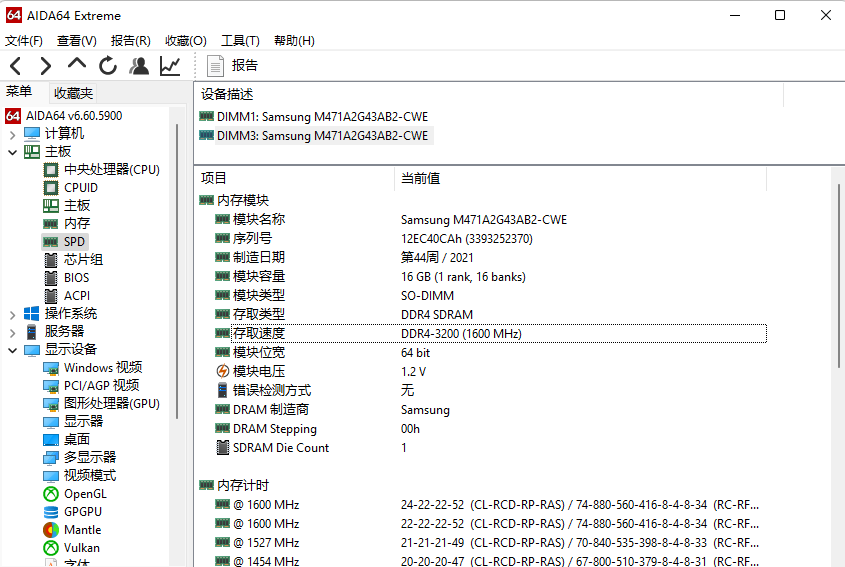
\includegraphics[width=\linewidth]{include_picture/spd_info.png}
    \caption{内存SPD信息} \label{spd_info}
  \end{subfigure}\\
\caption{内存信息} \label{mem_full_info}
\end{figure}

我使用相关软件查看了我自己设备的一些信息，图\ref{mem_info}中，我使用CPU-Z查看内存相关信息，可以看到我的两根内存条正确的组成了双通道，并且正常工作在1600MHz，由于DDR4内存在上升沿和下降沿均进行数据读写，所以数据读写频率3200MHz。然后我使用AIDA64软件查看内存SPD中的信息，可以看到模块位宽为64位。据此，我可以计算我内存的理论带宽上限：

$$3200MHz \times 64bit \times 2 = 51200MB/s$$

之后，我发现在AIDA64中也可以直接查询到主板内存总线的带宽，如图\ref{bus_info}所示，与上面的计算结果相符。此外，从图\ref{gpu_info}中可以发现，GPU的带宽为448.0GB/s，显然内存总线的带宽较低，可能成为瓶颈。不过实验一程序运行过程中，实际的传输速度比这个值还要小很多。

\begin{figure}[H] %H为当前位置，!htb为忽略美学标准，htbp为浮动图形
    \centering %图片居中
    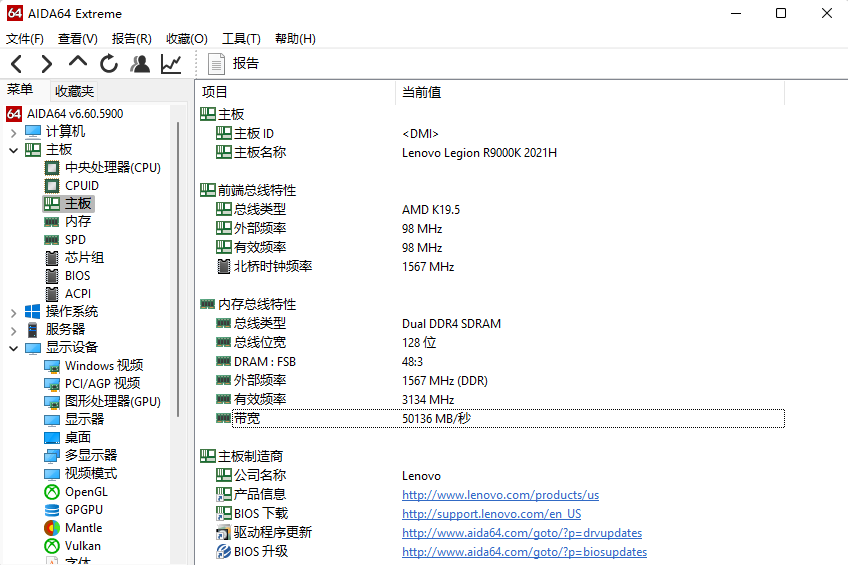
\includegraphics[width=0.8\textwidth]{include_picture/bus_info.png} %插入图片，[]中设置图片大小，{}中是图片文件名
    \caption{主板信息} %最终文档中希望显示的图片标题
    \label{bus_info} %用于文内引用的标签
\end{figure}

\section{实验二：并行前缀和}

该部分是作业中的第二个实验，同样用于帮助学生熟悉CUDA编程模型。实验一主要涉及到主机对于GPU核函数的调用，而实验二在实验一的基础上，还需要同学们自行进行串行算法设计，并编写核函数。虽然该实验名称为并行前缀和，但实际上该实验有两个部分，其中一个是并行前缀和，而另一部分是调用第一部分实现的并行前缀和，进一步实现查找数组中重复项的下标。

\subsection{实验背景}

并行前缀和算法是一种在并行计算中常用的技术，特别是在需要高效处理大数据集的场景中。它可以用来快速计算数组元素的累积和，以及在许多其他并行算法中作为基础步骤。查找数组中连续重复项的下标是一个典型的问题，可以通过并行前缀和算法来高效解决。

\subsection{实验代码浅析}

该实验核心代码均需要学生完成，因此只对代码文件做简单的介绍，不做过多赘述。

主程序main.cpp主要用于调用并行前缀和或查找重复项的算法实现，以完成指定的任务。任务由命令行参数指定，可以指定的内容包括但不限于：选择执行并行前缀和任务或者是查找重复项任务；选择不同的输入类型，默认为随机。scan.cu文件主要包括并行前缀和以及查找重复项的算法实现，这两部分都是需要学生完成的。

\subsection{实验过程}

\subsubsection{算法设计}

独占前缀和的算法实现参照实验说明中和课件中提供的算法，如图\ref{scan_algo}所示。该算法的伪代码也在实验说明中给出。该算法分为上扫和下扫两个阶段。在上扫阶段中，算法分组的收集元素的和，将其保存在固定的位置。具体来说，算法将每组中间的元素与最后的元素求和，并保存在组内最后的位置。组的长度从2开始，逐渐增加到不能覆盖完整数组的最大长度，也就是说，下一组参与求和的两个元素，恰好是上一组中保存两个和的两个元素。在下扫阶段，算法先将最后一个元素置零，然后将收集到的和分配到各个元素中。

\begin{figure}[H] %H为当前位置，!htb为忽略美学标准，htbp为浮动图形
    \centering %图片居中
    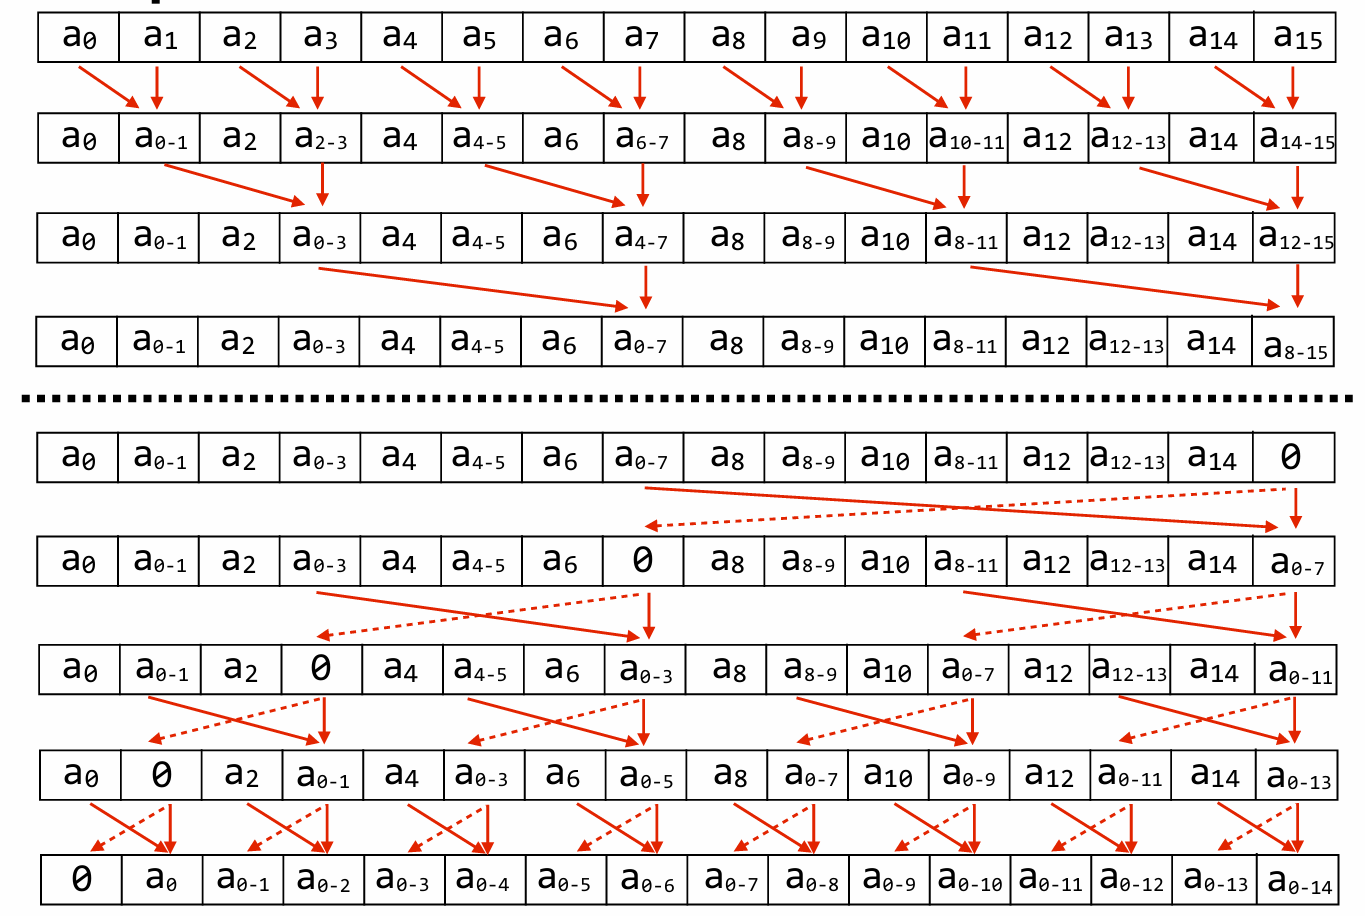
\includegraphics[width=0.8\textwidth]{include_picture/scan_algo.png} %插入图片，[]中设置图片大小，{}中是图片文件名
    \caption{并行独占和算法示意图} %最终文档中希望显示的图片标题
    \label{scan_algo} %用于文内引用的标签
\end{figure}

查找重复项的算法需要用到独占前缀和的计算，主要用后者实现对于下标的收集。具体的算法如图\ref{peak_algo}所示。具体来说，算法首先使用一个指示器，标记原始数组的某一元素是否与下一元素相同。然后对该指示器计算独占前缀和，用于表示前面已有重复项的数量，为最后一步并行的结果收集做指导。最后，检查独占前缀和中发生变化的项，其代表的就是这里有需要收集的下标，然后根据其内容，也就是表示前面已有的数量，将其放置在结果数组的对应位置中即可。总数可以使用最后一个元素的值来表示。

\begin{figure}[H] %H为当前位置，!htb为忽略美学标准，htbp为浮动图形
    \centering %图片居中
    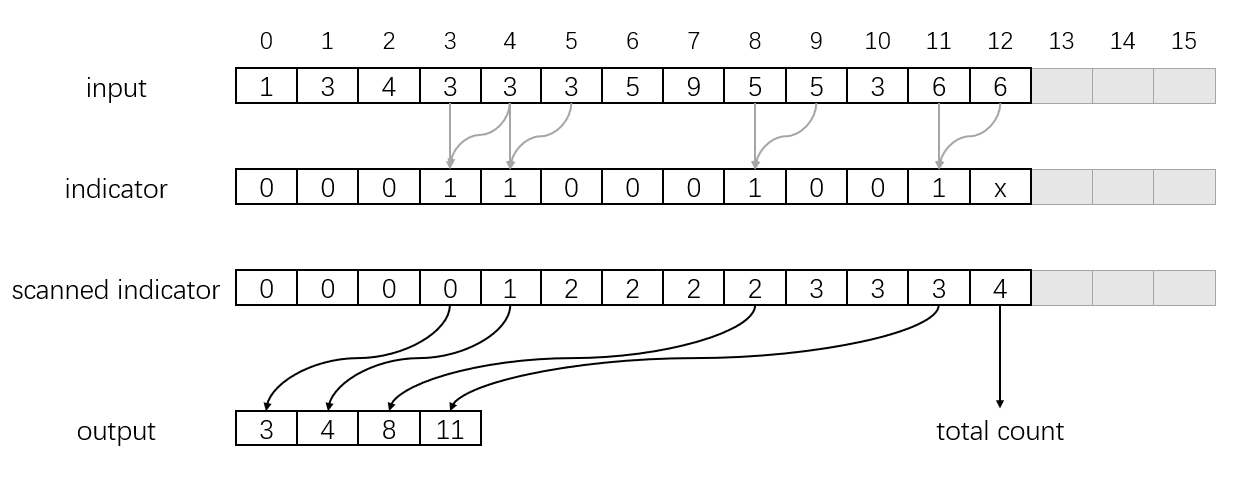
\includegraphics[width=0.8\textwidth]{include_picture/peak_algo.png} %插入图片，[]中设置图片大小，{}中是图片文件名
    \caption{查找重复项算法示意图} %最终文档中希望显示的图片标题
    \label{peak_algo} %用于文内引用的标签
\end{figure}

\subsubsection{实现过程}

该算法实现难度较低，依照算法与伪代码逐步实现即可。但在实现过程中，我也遇到了一些小问题，以下是实现独占前缀和的两个核函数，分别表示上扫阶段和下扫阶段。

\begin{lstlisting}[language=C++,title={独占前缀和核函数}]
__global__ void upsweep_kernel(const int two_d, const int two_dplus1, int * input, int * output, const int length) {
    int idx = (blockIdx.x * blockDim.x + threadIdx.x) * two_dplus1;
    if (idx < length) {
        output[idx + two_dplus1 - 1] = input[idx + two_dplus1 - 1] + input[idx + two_d - 1];
    }
}

__global__ void downsweep_kernel(const int two_d, const int two_dplus1, int * input, int * output, const int length) {
    int idx = (blockIdx.x * blockDim.x + threadIdx.x) * two_dplus1;
    if (idx < length) {
        // input maybe same with output
        int temp = input[idx + two_dplus1 \- 1];
        output[idx + two_dplus1 - 1] = input[idx + two_dplus1 - 1] + input[idx + two_d - 1];
        output[idx + two_d - 1] = temp;
    }
}
\end{lstlisting}

其中变量的命名与题目中的伪代码一致。其中，two\_dplus1表示组的长度，而two\_d表示组长度的一半，用于查找组中间的元素。在一开始编写核函数时，我忽略了input和output可能指向同一个地方，而在使用时我传入了相同的参数，导致了问题。

\subsection{结果与结论}

独占前缀和的实验结果如图\ref{scan_result}所示。可以看到性能超越了满分的要求。

\begin{figure}[H] %H为当前位置，!htb为忽略美学标准，htbp为浮动图形
    \centering %图片居中
    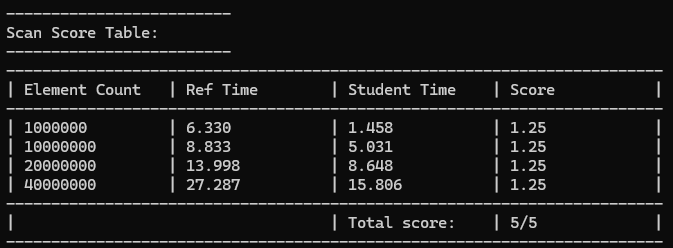
\includegraphics[width=0.8\textwidth]{include_picture/scan_result.png} %插入图片，[]中设置图片大小，{}中是图片文件名
    \caption{独占前缀和结果} %最终文档中希望显示的图片标题
    \label{scan_result} %用于文内引用的标签
\end{figure}

查找重复项的实验结果如图\ref{peak_result}所示。性能基本达到了满分的要求，只是在第一个小数据集上的性能没有达标。

\begin{figure}[H] %H为当前位置，!htb为忽略美学标准，htbp为浮动图形
    \centering %图片居中
    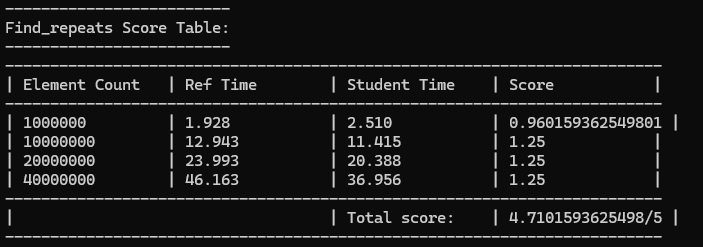
\includegraphics[width=0.8\textwidth]{include_picture/peak_result.png} %插入图片，[]中设置图片大小，{}中是图片文件名
    \caption{查找重复项结果} %最终文档中希望显示的图片标题
    \label{peak_result} %用于文内引用的标签
\end{figure}

据我分析，可能的原因主要有以下两个方面。一方面，我的算法实现局部性较差，对cache的利用率较为低下；同时在strided访存模式下，一次访问16字节数据，但仅使用4字节，同样降低了方寸效率，增加了访存次数。另一方面，该题本意可能是希望学生使用共享内存进行优化，这将带来显著的性能提升，尤其是在较小的数据集上。具体的原因可以使用NVIDIA Nsight Compute等工具进行进一步的分析。

\section{实验三：简单圆形渲染器}

该实验是本次作业最主要的内容，设计并实现一个CUDA并行圆形渲染器的渲染部分。

\subsection{实验代码浅析}

\subsubsection{代码概述}

该实验代码较多，分别位于许多不同的文件，包括但不限于以下文件。

首先是头文件。例如，circleRenderer.h声明抽象的CircleRenderer类，声明了一系列的虚函数，用于设置、动画、渲染等操作。cudaRenderer.h声明使用CUDA进行渲染的CudaRenderer类，refRenderer.h声明CPU渲染的RefRenderer类，它们都是CircleRenderer的派生类。cycleTimer.h声明用于高精度计时的CycleTimer类，主要用于性能测量；noise.h声明噪声生成函数；ppm.h声明用于写入PPM图像文件的函数；platformgl.h根据平台包含相应的GLUT库头文件，用于OpenGL编程；sceneLoader.h声明加载场景的函数；util.h声明一些实用宏和函数，例如颜色夹具函数CLAMP。

接着是一些cpp源文件。main.cpp是程序的主入口点，处理命令行参数，初始化渲染器，可以选择使用不同的渲染方式，处理不同的渲染任务。
当主程序使用渲染器时，首先调用allocOutputImage分配图像内存，然后使用loadScene来加载和初始化场景，接着调用setup进行初始化，最后由CheckBenchmark或其他函数，对每一帧图像调用clearImage、advanceAnimation和render来更新和渲染图像。display.cpp包含OpenGL渲染相关的代码，用于显示图像；noise.cpp实现噪声生成逻辑；ppm.cpp实现将图像数据写入PPM文件的逻辑；sceneLoader.cpp实现加载不同场景的逻辑。实验需要重点关注的也包括refRenderer.cpp，它实现RefRenderer类，是CPU渲染的参考实现。

然后是一些CUDA源文件。exclusiveScan.cu\_inl文件实现了一种用于CUDA中的独占前缀和操作的内联函数；benchmark.cu包含用于性能测试的CUDA代码。lookupColor.cu文件定义了一个用于在CUDA内核中查找颜色的设备内联函数，这个函数通过一个给定的坐标值在预定义的颜色映射表中进行插值，以获取对应的颜色值。noiseCuda.cu\_inl文件提供了一个在CUDA内核中生成噪声的设备函数。最后是最为核心的cudaRenderer.cu，这是一个不正确的并行CUDA实现，需要由学生修改完成。这个错误的实现不满足原子性和顺序要求，这点将在之后详细介绍。

此外，还有用于指导编译的Makefile以及用于测试的checker.py等文件，在实验过程中不需要过多关注。

\subsubsection{渲染过程浅析}

对于不同的场景，渲染器有着不同的帧更新逻辑，用于在渲染新的帧之前对元素进行调整。

而对于渲染过程，在串行实现中，任何场景的每个元素都会在render中被限定在一个矩形范围内，对于该范围内的任何一个像素，会被调用shadePixel进行真正像素的叠加。在这个函数里，位于矩形范围内，但在真正需要渲染的圆形范围外的像素会被忽略。对于雪花相关的场景，其像素颜色需要通过lookupColor进行颜色插值来获取，而其余场景则不需要，只需按照实验说明中的叙述，进行带有透明度的像素叠加即可。

在提供的错误CUDA实现中，渲染器将不同的圆圈分配给不同的线程，在每个线程中，通过两层循环来调用shadePixel，渲染各个圆形所在的矩形框中的像素。而此外，没有确保圆形渲染顺序的同步操作，或是对于某一像素的互斥访问，这也是导致这个实现不具备原子性和顺序性的原因。

\subsection{实验过程与结果}

在该实验中，我尝试了多个不同版本的实现。

在第一个版本中，我尝试使用像素级的并行，每个线程负责一个像素，按顺序处理所有的圆形。以下为这个基础版本的并行渲染核函数。

\begin{lstlisting}[language=C++,title={基础并行渲染核函数}]
__global__ void kernelRenderCircles() {
    short imageWidth = cuConstRendererParams.imageWidth;
    short imageHeight = cuConstRendererParams.imageHeight;
    short pixelX = blockIdx.x * blockDim.x + threadIdx.x;
    short pixelY = blockIdx.y * blockDim.y + threadIdx.y;

    // [0, imageWidth - 1], [0, imageHeight - 1]
    if (pixelX >= imageWidth || pixelY >= imageHeight) {
        return;
    }

    int circlesCnt = cuConstRendererParams.numCircles;
    // inverse coordinate
    float invWidth = 1.f / imageWidth;
    float invHeight = 1.f / imageHeight;
    float2 pixelCenterNorm = make_float2(invWidth * (static_cast<float>(pixelX) + .5f),
                                         invHeight * (static_cast<float>(pixelY) + .5f));
    float4 * imgPtr = (float4 *) (&cuConstRendererParams.imageData[(pixelY * imageWidth + pixelX) << 2]);

    for (int circleIdx = 0; circleIdx < circlesCnt; circleIdx++) {
        float3 circlePos = *(float3*)(&cuConstRendererParams.position[circleIdx * 3]);
        shadePixel(circleIdx, pixelCenterNorm, circlePos, imgPtr);
    }
}
\end{lstlisting}

在这个版本中，对于每个像素，同样也是每个线程，我计算了它在图像中的位置，计算像素中心点，然后在循环中调用shadePixel进行像素的更新。该版本的计时结果如图\ref{render_result1}所示，可以看到效率较低，与要求仍有较大差距。

\begin{figure}[H] %H为当前位置，!htb为忽略美学标准，htbp为浮动图形
    \centering %图片居中
    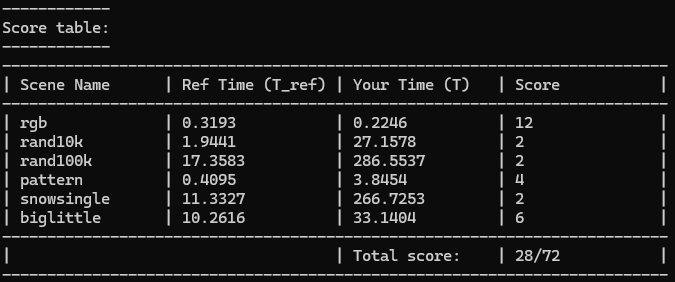
\includegraphics[width=0.8\textwidth]{include_picture/render_result_1.png} %插入图片，[]中设置图片大小，{}中是图片文件名
    \caption{渲染器结果1} %最终文档中希望显示的图片标题
    \label{render_result1} %用于文内引用的标签
\end{figure}

此时我注意到在shadePixel函数中有一个分支，对于每个像素的每个圆圈都会在GPU上进行执行，消耗时间较长，因此我决定尝试将这个分支移动到CPU上。在这个过程进行的同时，我拆开了shadePixel函数，将其逻辑直接写在圆形渲染函数中，并为两个不同的场景提供不同的圆圈渲染核函数，由CPU在调用渲染函数时就固定好分支，避免在GPU上执行分支操作，同时省略掉不必要的计算，并将本地使用局部变量保存各个像素的状态，减少对全局内存的访问。但当我完成一半，也就是完成对于通常场景的修改后，我发现这并没有什么作用，于是我放弃了我的修改。结合之后的实验，现在想来使用局部变量进行优化应该是有用的，但是对于分支的优化可能带来了意想不到的影响。后来我了解到了C++的constexpr，我使用它进行了优化，但出乎我意料的是，时间不仅没有缩短，某些场景下反而还显著增加了。经过我的测试，constexpr确实按照我的预期，将分支提前到了CPU上，且分支的次数也极大幅度的减小了，从每帧每像素每圆圈，减少到了每帧一次。所以执行时间的提升让我感到很不理解。图\ref{render_result2}展示了该情况下的耗时。

\begin{figure}[H] %H为当前位置，!htb为忽略美学标准，htbp为浮动图形
    \centering %图片居中
    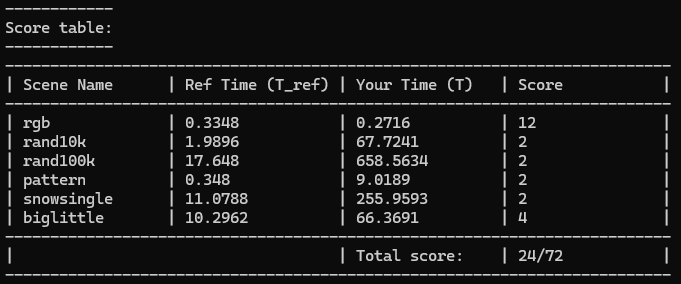
\includegraphics[width=0.8\textwidth]{include_picture/render_result_2.png} %插入图片，[]中设置图片大小，{}中是图片文件名
    \caption{渲染器结果2} %最终文档中希望显示的图片标题
    \label{render_result2} %用于文内引用的标签
\end{figure}

随后我开始思考如何优化算法，以获取更高的效率。我上网搜寻思路，意识到可以将像素分块处理，在每个块内仅处理与该块想交的圆圈，并将相交的圆圈信息保存在该块的共享内存中，以提升访存效率。在该算法中，每个线程块中的每个线程，不仅对应到具体的每个像素，还并行的查找相交的圆圈。具体来说，有一个每次处理块中线程数量圆的循环。在循环中首先，块中的各个线程根据当前块的范围，调用提供的函数circleInBoxConservative粗略的计算与自己对应的圆圈是否与该块相交，相交则标记指示器为1。然后与上一个实验类似，计算指示器的独占和，然后找到这一次循环中与该块相交的圆保存在共享内存中。接着各个线程代表各个像素，依次访问相交的圆，调用shadePixel更新像素。在这整个过程中，shadePixel更新的一直是本地的像素状态。当所有圆圈处理完成后，将其写回全局内存。该算法及其实现能够获得该实验的满分，结果见图\ref{render_result3}。

\begin{figure}[H] %H为当前位置，!htb为忽略美学标准，htbp为浮动图形
    \centering %图片居中
    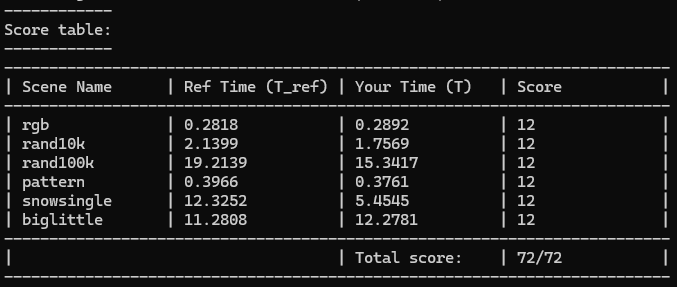
\includegraphics[width=0.8\textwidth]{include_picture/render_result_3.png} %插入图片，[]中设置图片大小，{}中是图片文件名
    \caption{渲染器结果3} %最终文档中希望显示的图片标题
    \label{render_result3} %用于文内引用的标签
\end{figure}

最后，我略微的进行最后的优化，调整了一些细节，进一步减少了对全局内存的访问，结果如图\ref{render_result4}所示，效果不太显著。

\begin{figure}[H] %H为当前位置，!htb为忽略美学标准，htbp为浮动图形
    \centering %图片居中
    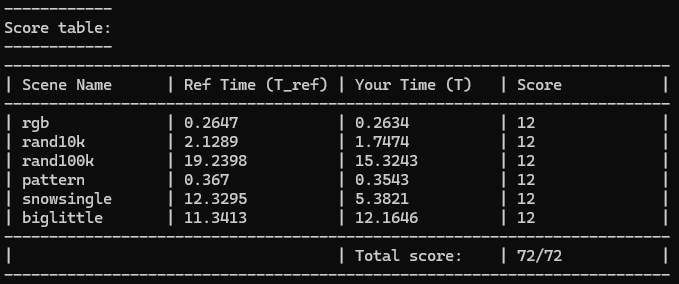
\includegraphics[width=0.8\textwidth]{include_picture/render_result_4.png} %插入图片，[]中设置图片大小，{}中是图片文件名
    \caption{渲染器结果4} %最终文档中希望显示的图片标题
    \label{render_result4} %用于文内引用的标签
\end{figure}

此外，如果将Position的三个值和半径合在一起，不仅能进一步减少访存，还能帮助16B对齐，进一步提高访存效率，但我没有实现这点。


\end{spacing}

\newpage

% XSP 2023/3/16: bib支持不全，暂时改为手动
\section*{参考文献} % section*生成无标号章节题目
\hypersetup{urlcolor=black}
\addcontentsline{toc}{section}{参考文献} % 将无标号章节添加至目录
% 著作: [序号]作者．书名[标识码]．出版地：出版社，出版年．
[1]NVIDIA A100 Tensor Core GPU Architecture. Available: \url{https://images.nvidia.com/aem-dam/en-zz/Solutions/data-center/nvidia-ampere-architecture-whitepaper.pdf}

[2]Nvidia Hopper Architecture New Features. Available: \url{https://zhuanlan.zhihu.com/p/676437405}

[3]Work-efficient parallel exclusive scan (O(N) work). Available: \url{https://gfxcourses.stanford.edu/cs149/fall23/lecture/dataparallel/slide_16}

[4]CMU 15418 Spring 2023 Assignment 2: A Simple CUDA Renderer. Available: \url{https://zhuanlan.zhihu.com/p/683223356}

% \begingroup
% \setstretch{2.0}    %行距2
% \setlength{\bibsep}{0pt}    %段前段后0
% \begin{adjustwidth}{0.42cm}{0.42cm} %左右缩进0.42cm
% \bibliography{references}
% \end{adjustwidth}
% \endgroup

\end{document}
